\chapter{Web scraping, extracción de datos en la web}
\label{cha:web scraping, extraccion de datos en la web}

\section{En que consiste realmente el web scraping}
\label{sec:en que consiste realmente el web scraping}

En la actualidad el \emph{web scraping} se puede definir como una \emph{“solución tecnológica para extraer
información de sitios web, de forma rápida, eficiente y automática, ofreciendo datos en un formato más
estructurado y más fácil de usar \cite{web-scraping-osmar-castrillo}”}. Sin embargo, esta definición no ha
sido siempre así, los métodos de minado web han evolucionado desde procedimientos más pequeños con ayuda
humana, hasta sistemas automatizados capaces de convertir sitios web completos en conjuntos de datos bien
organizados.

Existen diferentes herramientas de minado, no solo capaces de analizar los lenguajes de marcado o archivos
JSON, también capaces de realizar un procesamiento del lenguaje natural para simular cómo los usuarios
navegan por el contenido web.

\subsection{Extracción de los datos}
\label{subsec:extraccion de los datos}

En realidad el minado web es una práctica muy sencilla, se extraen datos de la web y se almacenan en una
estructura de datos para su posterior análisis o recuperación. En este proceso, un agente de software,
también conocido como robot, imita la navegación humana convencional y paso a paso accede a tantos sitios
web como sea necesario \cite{web-scraping-api-world}. Las fases por las que pasa el agente software en
cuestión se determinan a continuación:

\begin{enumerate}
\item {\bfseries Fase de búsqueda:} Esta primera fase consiste en el acceso al sitio web del que se
quiere obtener la información. El acceso se proporciona realizando una solicitud de comunicación HTTP.
Una vez establecida la comunicación, la información se gestiona a partir de los métodos GET y POST usuales.

\item {\bfseries Fase de extracción:} Una vez que el acceso ha sido permitido, es posible obtener la
información de interés. Se suelen emplear para este propósito expresiones regulares o librerías de
análisis HTML. Los diferentes softwares empleados para este propósito se especifican en la sección
\ref{subsec:herramientas software disponibles}.

\item {\bfseries Fase de transformación:} El objetivo de esta fase es transformar toda la información
extraída en un conjunto estructurado, para una posible extracción o análisis posterior. Los tipos de
estructuras más comunes en este caso son soluciones basadas en cadenas de texto o archivos CSV y XML.
\end{enumerate}

Una vez que el contenido ha sido extraído y transformado en un conjunto ordenado, es posible realizar un
análisis de la información de una forma más eficaz y sencilla que aplicando el método tradicional. El
proceso descrito se resume en la ilustración \ref{img:web-scraping-phases}.

\begin{figure}[tphb]
\centering
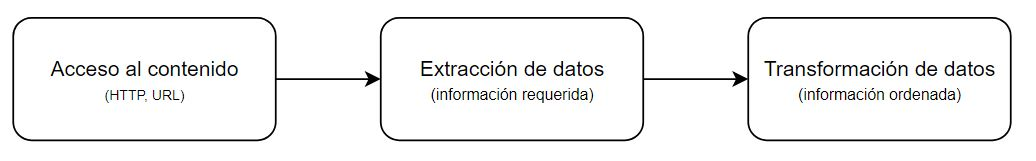
\includegraphics[width=6in]{web-scraping-phases.jpg}
\caption{Fases del web scraping}
\label{img:web-scraping-phases}
\end{figure}

Por otro lado, a lo largo del apéndice \ref{cha:funcionamiento basico de un web scraper}, se ilustra el
funcionamiento del agente software en cada una de las fases descritas anteriormente, así como de su
comportamiento con el servidor web al que se desea acceder.

\subsection{Herramientas software disponibles}
\label{subsec:herramientas software disponibles}

El software disponible que emplean los \emph{web scrapers} puede dividirse en varios enfoques, ya sean 
bibliotecas de programación de propósito general, \emph{frameworks}, o entornos de escritorio.

Por lo general tanto los \emph{frameworks} como los entornos de escritorio presentan una solución más 
sencilla e integradora con respecto a bibliotecas de programación. Esto es debido a que ambos, no se ven 
afectados a los posibles cambios HTML de los recursos a los que accede. Además, estas necesitan la 
integración de otras múltiples bibliotecas adicionales para el acceso, análisis y extracción del contenido.

Este trabajo se desarrolla sobre bibliotecas de programación, las cuales se implementan como un programa
software convencional utilizando estructuras de control y de datos del propio lenguaje. Por lo general,
bibliotecas como \emph{curl \cite{curl-cran}} conceden acceso al sitio web deseado haciendo uso del
protocolo HTTP, mientras que los contenidos extraídos se analizan a través de funciones como la
coincidencia de expresiones regulares y la tokenización.

Comprender como las bibliotecas obtienen los datos de los sitios web, pasa por conocer las diferentes
formas en las que los documentos HTML se organizan. Existen dos técnicas, dependiendo si se realiza un
renderizado previo o no \cite{tfg-daniel-francisco-lopez}. La primera técnica consiste simplemente en
parsear, es decir, realizar un análisis léxico-sintáctico sobre estructuras XML o HTML. Se suelen emplear
expresiones XPath o selectores CSS para su realización. Por otro, lado si es necesario que parte de la 
lógica del sitio web pase al lado del cliente, este deberá pasar por un proceso de renderizado previo.

Con el paso del tiempo, cada vez se extiende más el uso de bibliotecas de desarrollo como JQuery, encargadas 
de pasar parte de la lógica del lado del servidor al lado del cliente con el objetivo de favorecer la 
interactividad. Estas páginas no podrán ser analizadas si no se renderizan antes.

\subsubsection{XPath}
\label{subsubsec:xpath}

XPath es un lenguaje que permite construir expresiones que recorren y procesan un documento XML
\cite{css-xpath-lilland}. Puede utilizarse para navegar por documentos HTML, ya que este es un lenguaje
similar en cuanto a estructura a XML. Es comúnmente utilizado en el \emph{web scraping} para extraer datos 
de documentos HTML, además utiliza la misma notación empleada en las URL para navegar por la estructura 
del sitio web en cuestión.

\subsubsection{Selectores CSS}
\label{subsubsec:selectores CSS}

El segundo método de extracción de datos en documento HTML se realiza a través de lo que se conoce como
selectores CSS \cite{css-xpath-lilland}. CSS es el lenguaje utilizado para dar estilo a los documentos
HTML, por otro lado, los selectores son patrones que se utilizan para hacer coincidir y extraer elementos
HTML basados en sus propiedades CSS.

Hay múltiples sintaxis de selector diferentes, estas se corresponden con la forma en la que el documento
CSS está estructurado. En el fragmento de código \ref{cod:extraccion de datos de interes del documento}
se hace uso de los selectores \emph{'.text-primary'} y \emph{'.lister-item-header a'} para acceder al
contenido web deseado.

\subsection{Tipologías}
\label{subsec:tipologias}
Dependiendo de como se acceda y extraiga la información, existen dos técnicas de \emph{web scraping}. Se 
mencionan los siguientes supuestos a continuación:

\begin{itemize}
\item Si la información que se almacena no procede de sitios web concretos, sino que durante el análisis
de páginas web se encuentran enlaces que retroalimentan el análisis de otras nuevas, el método se conoce
como \emph{web crawling} \cite{Andreas-Mehlfuhrer}.

\item Por el contrario, si la información se extrae de sitios web concretos, donde ya se conoce como extraer 
y generar un valor por la misma, la técnica se conoce como \emph{web scraping} genérico. Mientras que en 
el \emph{web crawling} el resultado de ejecución es la obtención de nuevas páginas, en el \emph{web scraping} 
el resultado es la propia información.
\end{itemize}

Es decir, la principal diferencia entre ambas, es que mientras los \emph{web scrapers} extraen información 
de páginas webs concretas, los \emph{web crawlers} almacenan y acceden a las páginas a través de los enlaces
contenidos en las mismas. En la figura \ref{img:web-scraping-phases} se mostraba la arquitectura en fases
de un \emph{web scraper}, veamos a continuación como es la arquitectura de un \emph{web crawler}.

\begin{figure}[tphb]
\centering
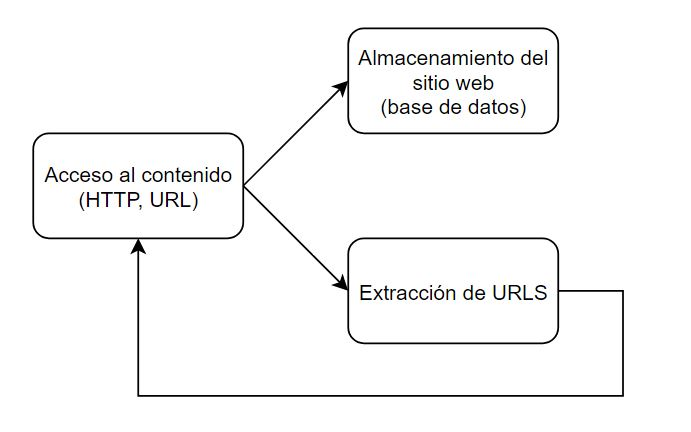
\includegraphics[width=4in]{web-crawler-phases.jpg}
\caption{Fases del web crawling}
\label{img:web-crawler-phases}
\end{figure}

Ya sea empleando cualquiera de estas dos tipologías, existen páginas que no pueden ser analizadas o
rastreadas. Esto es debido a que algunos sitios web solo están disponibles con una autorización previa, o
necesitan información especial para su acceso.

\section{Posibilidades prácticas del web scraping}
\label{sec:posibilidades practicas del web scraping}

Son muchas las aplicaciones prácticas de la minería web, la mayoría de estas entran en el ámbito de la
ciencia de los datos. En la siguiente lista se exponen algunos casos de su uso en la vida real
\cite{web-scraping-seppe}:

\begin{itemize}
    \item Bancos y otras instituciones financieras utilizan minería web para analizar a la competencia.
    Inversores también utilizan \emph{web scraping}, para hacer un seguimiento de artículos de prensa 
    relacionados con los activos de su cartera.

    \item En las redes sociales se emplea minería de datos para conocer la opinión de la gente a cerca de 
    un determinado tema.

    \item Existen aplicaciones capaces de analizar diferentes sitios web y encontrar los mismos productos 
    a precio reducido. Incluso capaces de detectar ofertas de artículos a tiempo récord.

    \item etcétera
\end{itemize}

El minado web contiene infinidad de aplicaciones, muy diversas e interesante capaces de automatizar el
trabajo y conseguir la información de forma ordenada. No obstante, muchos sitios web ofrecen alternativas 
como el uso de APIs o ficheros estructuras para el acceso a dichos datos. 

En general el \emph{web scraping} es una técnica que consume bastantes recursos, por lo que el desarrollador 
debe limitar su uso si existen otras alternativas, como las APIs, que proporcionan los mismos resultados.

\section{Retos del web scraping}
\label{sec:retos del web scraping}

La forma en la que se crean los sistemas de extracción web se ha discutido desde diferentes perspectivas
a lo largo del tiempo. Se emplean métodos científicos como el aprendizaje automático, la lógica o el
procesamiento del lenguaje natural para lograr su implementación.

Uno de los principales retos a afrontar tiene relación con las fuentes cambiantes de información. A menudo,
una herramienta de extracción tiene que obtener datos de forma rutinaria de una determinada página o sitio
web que puede evolucionar con el tiempo. Estos cambios se producen sin previo aviso, son imprevisibles,
por lo que es bastante probable que los raspadores web se vean sometidos a cambios. Por ello, surge la
necesidad crear herramientas flexibles capaces de detectar y afrontar modificaciones estructurales de las
fuentes web relacionadas.

Otros problemas recaen sobre la información extraída. En primer lugar, uno de los aspectos que se deben
tener en cuenta al obtener información trata sobre la fiabilidad de la misma. Aunque la información
exista y se pueda ser analizada, esta puede que no sea correcta. La gramática y la ortografía pueden ser
un problema en la fase de análisis, ya que información puede perderse o ser falsamente recogida. Por otro
lado, tanto aplicaciones que tratan con datos personales, como software de minado deben ofrecer garantías
de privacidad. Por lo tanto, los posibles intentos de violar la privacidad del usuario deben ser
identificados y contrarrestados a tiempo y de forma adecuada.

Puesto que multitud de técnicas de minería web requieren ayuda humana, un primer reto consiste en
proporcionar un alto grado de automatización, reduciendo así al máximo el esfuerzo humano. Sin embargo,
la ayuda humana puede desempeñar un papel importante a la hora de elevar el nivel de precisión alcanzado
por un sistema de extracción de datos web, por ello la clave está en encontrar un equilibrio entre
automatización e intervención humana.

Por último, a pesar de que las herramientas de \emph{web scraping} han evolucionado con el tiempo, los 
aspectos legales están algo inexplorados pues dependen de los términos y condiciones de cada sitio web en 
cuestión.

\section{Aspectos ético-legales del web scraping}
\label{sec:aspectos etico-legales del web scraping}

Para comprender los aspectos legales del \emph{web scraping}, debemos recordar el robot o agente software
definido en el apartado \ref{subsec:extraccion de los datos}. Este agente software, previamente examinado 
por el servidor, es el que se encarga de acceder y realizar un recorrido por el contenido web.

Durante el acceso al contenido, se espera que este agente se ajuste a los términos de uso del sitio en
cuestión, así como el cumplimiento del archivo \emph{'robots.txt'} \footnote{Archivo alojado en el
servidor web, que gestiona el tráfico del mismo e indica los documentos a los que no se debe acceder de
forma automática \cite{robots-txt}.}, con el objetivo de evitar accesos no deseados y sobrecargas en el
servidor.

Puesto que el documento \emph{'robots.txt'} no es de obligado cumplimiento, a lo largo de los años la
reputación del \emph{web scraping} ha decrecido de forma significativa. Muchos agentes software no siguen 
las indicaciones determinadas, por lo que definir la cantidad de accesos y archivos a los que se accede
dependerá de la ética de cada desarrollador.

Con el objetivo de tener una cierta garantía de que nuestro agente software cumple con los aspectos
ético-legales, se deben tener en consideración las siguientes cuestiones \cite{legalidad-web-scraping}:

\begin{itemize}
    \item Leer los términos de uso de la página web en al que se vaya a realizar el minado.

    \item Inspeccionar y cumplir con el documento robots.txt, para ser capaces de identificar los accesos
    del servidor.

    \item Realizar peticiones al servidor de forma controlada. Puede que el índice de solicitudes al 
    servidor no este especificado en el documento, si esto sucede debemos determinar un número de solicitudes 
    razonable, por ejemplo, una solicitud por segundo.
\end{itemize}

















